\documentclass{mbd_fullpaper}

\begin{document}

%New commands
\newcommand{\heading}[1]{
   {\medskip\hskip5em\bf\large{#1}
   \vskip0.5ex
   }
}
\newcommand{\eqnref}[1]{
  (\ref{#1})
}

\renewcommand{\refname}{\medskip\bf\large References}



%------------------------------------------------------------
% title
\begin{center}
  \Large{\bf
Equivalent Mass-Spring Models of Multibody Spacecraft for the Application of Wave-based Control  }
\end{center}

%------------------------------------------------------------
% authors
\begin{center}
\large{
Joseph W. Thompson
}
\end{center}

%------------------------------------------------------------
% affiliations
{
\begin{center}
 \small
  \begin{tabular}{c}
    School of Mechanical and Materials Engineering \\
    University College Dublin              \\
    Belfield, Dublin 4, Ireland        \\
    joseph.thompson@ucdconnect.ie                        \\
  \end{tabular}
\end{center}
}

%------------------------------------------------------------
% abstract



\section*{Abstract}
% It contains a general introduction to the topic, outlines the major results, and summarizes the conclusions.
% 250 words max.

%Wave-Based Control (WBC) is particularly effective for achieving rest to rest motion of under-actuated, cascaded, lumped flexible systems.
%In this control scheme the actuator simultaneously launches and absorbs wave components travelling into and out of the system at one end.
%By doing this the control scheme combines position control and active vibration damping.
%Much work has been done on wave-based modelling and control of mass-spring strings.
%This paper asks the question: to what extent can this work be extended to a wider class of systems?
%This question is motivated by the control of spacecraft with features such as structural flexibility, flexible appendages and fuel slosh.
%Most mathematical models of these systems presented to the control engineer, do not obviously have the structure of a mass-spring string.
%However, often it is possible to calculate an equivalent mass-spring system.
%This paper identifies a class of systems, with real, positive and distinct eigenvalues, for which this transformation is possible and presents an algorithm for calculating the equivalent mass and spring values.
%A segmented planar multibody rocket model is used as an example.
%This model consists of three rigid bodies connected by two torsional springs and a gimballed rocket engine with constant thrust which may be used for attitude control.
%Several test cases with different sensor and actuator configurations are examined and equivalent mass-spring systems are calculated in each case.

\keywords{multibody spacecraft, attitude control, mechanical waves, vibration, lumped systems}

\section{Introduction}
% The first paragraph should follow the inverted triangle principle: start with a broad statement and
% become more detailed until finally identifying the specific problem that the paper addresses.
Many spacecraft and rockets may be modelled as multi-body systems \cite{kane}.
Flexible structures such as solar panels, or robot arms, may be approximated by a lumped equivalent - a number of joined rigid bodies, with springs in each joint.
Sloshing fuel may be represented by a simple pendulum or a mass-spring analog.
These simple representations are particularly useful in the design of an attitude controller.
These systems are usually under-actuated i.e. have more degrees of freedom than actuators.
In attempting to re-orient such a system, one will usually excite certain modes of vibration.
To bring the system back to rest, the control algorithm must effectively dampen these vibrations.
To end up with the correct target attitude at the end of a manoeuvre this exciting and damping of vibrations must be done in precisely the right way.
One possible approach to this problem is to model the motion of each part of the system as a superposition of two components or `waves'.
One wave is travelling from the actuator into the system and the other is travelling from the system back towards the actuator.
In this way the actuator is simultaneously launching a wave into the system and absorbing a returning wave from the system.
A complete manoeuvre consists of launching a certain wave into the system and then absorbing the returning wave to bring the system back to rest.
The above wave-based control technique has been applied successfully to uniform and non-uniform rectilinear mass-spring systems.
The aim of this paper is to extend the wave-based control theory to a wider class of systems, namely the multi-body spacecraft described above. 

\begin{figure}[h]
  \begin{center}
    	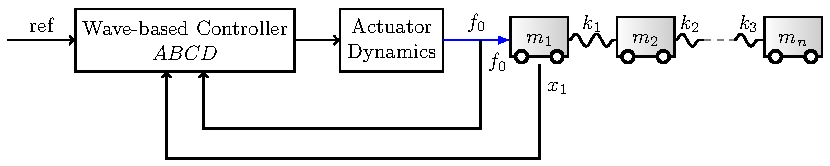
\includegraphics[scale=1]{graphics/WBC-nunif-mspring-force.pdf}
    	%%Styles
\tikzstyle{block} = [draw, thick, rectangle, minimum height=3em, minimum width=3em]
\tikzstyle{math} = [draw, thick, circle, minimum size=0.6cm,node distance=2cm, path picture={ 
      \draw[line] (path picture bounding box.south west) -- (path picture bounding box.north east);
      \draw[line] (path picture bounding box.north west) -- (path picture bounding box.south east);}]
\tikzstyle{gain} = [draw, thick, isosceles triangle, minimum size=0.6cm,node distance=1.5cm]
\tikzstyle{pt} = [coordinate]
\tikzstyle{line} = [->,thick]
\tikzstyle{ground}=[color=gray,postaction={draw,decorate,decoration={border,angle=-45,amplitude=0.2cm,segment length=2mm}}]
\tikzstyle{actuator} = [draw=blue!50!black ,fill=blue!50!black!50!white, thick, rectangle, inner sep=0,minimum height=0.6cm, minimum width=0.2cm, node distance=1.8cm]
\tikzstyle{spring} = [thick,black,decorate,decoration={snake,amplitude=3,segment length=10}]
\tikzstyle{wheel} = [thick,orange,decorate,decoration={coil,aspect=0.7,amplitude=5}]
\tikzstyle{cart} = [rectangle, inner sep=0,minimum height=0.8cm, minimum width=1cm, node distance=1.8cm, path picture={ 
      \shadedraw[left color=white,right color=gray!40!white, thick] ([yshift=0.12cm, xshift=0.3pt] path picture bounding box.south west) rectangle ([xshift=-0.3pt,yshift=-0.3pt] path picture bounding box.north east); 
      \draw[very thick, fill=white] ([yshift=0.12cm, xshift=-0.3cm] path picture bounding box.south) circle (0.1cm);
      \draw[very thick,fill=white] ([yshift=0.12cm, xshift=0.3cm] path picture bounding box.south) circle (0.1cm);}]
\tikzstyle{pt} = [coordinate]
\tikzstyle{force}=[->,thick,>=latex,draw=blue,fill=blue]

\begin{tikzpicture}[auto]

%Nodes
	\node[pt]	at (0,0)	(ref)													{};
	\node[block] 		(con) 		[right of=ref, node distance=3cm, align=center] 		{Wave-based Controller \\ $A B C D$};
	\node[block] 		(act) 		[right of=con, node distance=3.5cm, align=center]  		{Actuator \\ Dynamics};
	\node[pt]			(for)		[right of=act, node distance=1.5cm]							{};

	
	\node[cart]	(m1)		[right of=for, node distance=1cm]			{$m_1$};
	\node[cart] 	(m2) 		[right of=m1] 	{$m_2$};
	\node[pt] 	(pt1) 		[right of=m2, node distance=1cm] 	{};
	\node[pt] 	(pt2) 		[right of=pt1, node distance=0.5cm] 	{};
	\node[cart] 	(m3) 		[right of=pt2, node distance=1cm] 	{$m_n$};
 	
 	\node[pt]			(int)		[below of=m1, node distance=2cm]							{};
 	\node[pt]			(int2)		[below of=for, node distance=1.5cm]							{};
 	
%Connections	
      \draw[force] (act) -- node {$f_0$} (m1);
 	\draw[line] (ref) -- node {ref}  (con);
 	\draw[line] (con) -- (act);
	\draw[line] (m1) -- node[near start] {$x_1$} (int) -| (con.240);
	\draw[line] (for) -- node[near start] {$f_0$} (int2) -| (con.300);
% 	\draw[line] (minus_x0) -- (k0);
% 	\draw[line] (k0) -- node[] (N2) {$M_{ref}$} (m1);
	
	\draw[spring] (m1) -- node[above] {$k_1$} (m2);
	\draw[spring] (m2) -- node[above] {$k_2$} (pt1);
	\draw[thick,gray, dashed] (pt1) -- (pt2);
	\draw[spring] (pt2) -- node[above] {$k_3$} (m3);
	%\draw[ground] (m1.south west) -- (m3.south east);

\end{tikzpicture}
	\caption{Wave-based-control scheme for a mass-spring string \label{fig:wave-based-control}}
  \end{center}
\end{figure}
Figure \ref{fig:wave-based-control} shows a simple wave-based control system.
The generic mass-spring string shown is a classical example of an under-actuated control problem.
The motion of this lumped system may be modelled as a superposition of two "waves" or wave-like components travelling rightwards and leftwards\cite{OConnor2011}.
Using this wave-based interpretation of the system, linear controllers have been designed with a number of desirable properties \cite{Connor2005}. 
These include robustness to modelling errors, system changes, sensor delays and non-ideal actuation, minimal sensing and ease of implementation.
These controllers operate as follows: The initial movement of the actuator $x_0$ launches a wave (motion which propagates rightwards through the string) which reaches the system boundary and is reflected.
After reflection the motion (returning wave) travels leftwards back to the actuator which moves to absorb it.
This returning wave is resolved using two measurements from the system.
These measurements can be positions, velocities or forces and are usually taken close to the actuator.
In Figure \ref{fig:wave-based-control} these measurements are the position of the first mass $x_1$ and the force being applied to the first mass $f_0$.
In addition to the mass-spring shown in Figure \ref{fig:wave-based-control} this type of controller has been applied to a much wider array of systems. (citations)
However in these cases the approach to controller design and tuning has been experimental in nature and the underlying waves are not clearly defined.
It is proposed here that many of these more complicated systems are in fact similar in structure to the mass-spring system in Figure \ref{fig:wave-based-control}.
Furthermore it is proposed that through a suitable change of coordinates, an equivalent mass-spring string may be calculated for many of these systems.
Given a SISO (single-input single-output) undamped system described by:
\begin{equation}
\ddot{\mathbf{q}}(t) + \Lambda\mathbf{q}(t) = \mathbf{b}u(t)
\label{eq:modal1}
\end{equation}
\begin{equation}
y(t) = \mathbf{c}^T \mathbf{q}(t)
\label{eq:modal2}
\end{equation}
where
\begin{equation}
\Lambda = \begin{bmatrix}
\lambda_1  &  0 & \cdots & 0 \\
0 & \lambda_2  & \ddots & 0 \\
\vdots & \ddots & \ddots & \vdots \\
0 & 0 & \cdots & \lambda_n \end{bmatrix}
,\quad \mathbf{b} = \begin{bmatrix} b_1 \\ b_2 \\ \vdots \\ b_n \end{bmatrix}
,\quad \mathbf{c} = \begin{bmatrix} c_1 \\ c_2 \\ \vdots \\ c_n \end{bmatrix}
\end{equation}
where $u(t)$ is the input and $y(t)$ is the output, this leads to the following problem statement:
\begin{enumerate}
\item under what conditions can this system be transformed into an equivalent mass-spring string such as in Fig.1 (for which WBC is known to work well) and
\item how can the parameters of this equivalent system be calculated?
\end{enumerate}
The problem becomes if (and if so, how) we can find a coordinate transformation $\mathbf{x} = P \mathbf{q}$ such that:
\begin{equation}
M\ddot{\mathbf{x}}(t) + K\mathbf{x}(t) = \mathbf{\hat{b}}u(t)
\label{eq:eom1}
\end{equation}
\begin{equation}
y(t) = \mathbf{\hat{c}}^T \mathbf{x}(t)
\label{eq:eom2}
\end{equation}
and $M$, $K$, $\mathbf{\hat{b}}$ and $\mathbf{\hat{c}}$ have the following structure:
\begin{equation}
M = \begin{bmatrix}
m_1  &  0 & \cdots & 0 \\
0 & m_2  & \ddots & 0 \\
\vdots & \ddots & \ddots & \vdots \\
0 & 0 & \cdots & m_n \end{bmatrix}
, \quad
K = \begin{bmatrix}
k_1+k_2  &  -k_2 & 0 & \cdots & 0 \\
-k_2 & k_2+k_3  & -k_3 & \ddots & 0 \\
0 & -k_3 & \ddots & \ddots & \vdots \\
\vdots & \ddots & \ddots & k_{n-1}+k_n & -k_{n} \\
0 & 0 & \cdots & -k_{n} & k_n \end{bmatrix}
,\quad \mathbf{\hat{b}} = \begin{bmatrix} {1}/{m_1} \\ 0 \\ \vdots \\ 0 \end{bmatrix}
,\quad \mathbf{\hat{c}} = \begin{bmatrix} 1 \\ 0 \\ \vdots \\ 0 \end{bmatrix}
\end{equation}

%The introduction ends with the “road-map” paragraph. This paragraph outlines the remaining sections of the paper. It can either give a general outline of the contribution,
%or a specific, section-by-section breakdown of the remaining article.
Road map
Section 2 - WBC control system
Section 3 - Mathematical model of segmented rocket
Section 4 - Class of systems to which WBC can be applied, and algorithm for converting to standard mass-spring form
An algorithm is developed to find a suitable coordinate transformation $\mathbf{z} = P \mathbf{q}$ to achieve this objective.
The problem may be first reduced to an inverse eigenvalue problem for a Jacobi matrix. This may be solved using the Lanczos algorithm as presented in \cite{gladwell1986inverse}. 
It is found that there are many equivalent mass-spring systems depending on the desired forms of the input vector $\hat{\mathbf{b}}$ and output matrix $\hat{C}$, that is, on the input-output structure of the system or the location(s) of actuators and sensors in the string.
Section 5 - Numerical Examples - different position of sensors, actuators
Section 6 - Discussion
Section 7 - Conclusions 

\section{Transformation to equivalent mass-spring model}
This section outlines the process for converting
We restrict ourselves to the case where the eigenvalues are real and distinct, i.e.
\begin{equation}
0 \leq \lambda_1<\lambda_2< \cdots <\lambda_n
\label{eq:lambda}
\end{equation}

\section{Wave-Based Control Scheme}
The details of the wave-based control scheme
linear controller
State space system
tuning parameters w and k0
choose w from k1 m1

\section{Mathematical Model of Segmented Rocket}
In this section the equations of motion for a planar segmented rocket are presented.
Why pick this model
It should be noted that even though this is a lumped model with three bodies and two springs, the dynamics of this system are quite different from that of a simple rectilinear 3-mass, 2-spring system and the subtle differences, which will become clear in subsequent sections are what motivate the current study.
Also note that from control point of view it is inputs and outputs that are important
When sensor is at top how can we apply WBC theory.

The model consists of three rigid bodies connected by two torsional springs as shown in figure \ref{fig:rocket-model}.

\begin{figure}[h]
  \begin{center}
    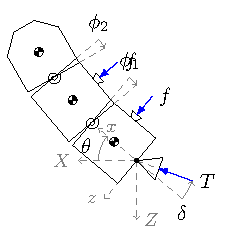
\includegraphics[scale=1]{graphics/seg3-rocket-allact.pdf}
    \caption{Segmented planar rocket model \label{fig:rocket-model}}
  \end{center}
\end{figure}
The attitude of the bottom or base segment is $\theta$ relative to an inertial reference frame.
The middle and top segments have angles $\phi_1$ and $\phi_2$ respectively between themselves and the segment below as shown.
Each segment has has height $h$, mass $m$ and moment of inertia $I$ about its mass centre and each torsional spring has stiffness $k$.
The rocket is considered to have four possible sources of actuation: a lateral force $f_i$ at the mass centre of each of the three segments, and a moment on the bottom segment as shown.
This combination of inputs allow many different cases to be considered, for example if the actuator is a gimballed engine at the bottom then the input to the system will be a combination of force $f_1$ and moment $M$.
The equations of motion of the system were derived using Kane's method \cite{Kane1980} and linearised about the equilibrium point $\theta=\dot{\theta}=\phi_i=\dot{\phi}_i=0$
\begin{equation}
\end{equation}
where
\begin{equation}
\input{python/eqM.tex}
\end{equation}
Different actuators
figure

\section{Numerical Examples}
Physical parameters vega
Note: ignoring aerodynamics and gravity, for demonstration purposes only!
Several models defined by different sensor actuator configs
Conversion to equivalent mass-spring model
1
2
3
4
Simulations
Step responses

\section{Discussion}
Is conversion possible, when is possible
Still a large class of systems

Mass Spring ratios, uniformity better
for that rocket model sensor at bottom is better
Wave-based intuition behind this. Longer settling time for actuator at top
System tells us best location for actuator
Future work, use this to optimise actuator and sensor location

\section{Conclusions}


%------------------------------------------------------------
% biliography
\bibliographystyle{acm}
\bibliography{eccomas_2017}

\end{document} 
